\usetikzlibrary{calc,matrix,shapes,positioning,fadings}

\tikzfading[name=fade out,
inner color=transparent!0,
outer color=transparent!100]


\newcommand{\convexpath}[2]{
[   
    create hullnodes/.code={
        \global\edef\namelist{#1}
        \foreach [count=\counter] \nodename in \namelist {
            \global\edef\numberofnodes{\counter}
            \node at (\nodename) [draw=none,name=hullnode\counter] {};
        }
        \node at (hullnode\numberofnodes) [name=hullnode0,draw=none] {};
        \pgfmathtruncatemacro\lastnumber{\numberofnodes+1}
        \node at (hullnode1) [name=hullnode\lastnumber,draw=none] {};
    },
    create hullnodes
]
($(hullnode1)!#2!-90:(hullnode0)$)
\foreach [
    evaluate=\currentnode as \previousnode using \currentnode-1,
    evaluate=\currentnode as \nextnode using \currentnode+1
    ] \currentnode in {1,...,\numberofnodes} {
-- ($(hullnode\currentnode)!#2!-90:(hullnode\previousnode)$)
  let \p1 = ($(hullnode\currentnode)!#2!-90:(hullnode\previousnode) - (hullnode\currentnode)$),
    \n1 = {atan2(\y1,\x1)}, 
    \p2 = ($(hullnode\currentnode)!#2!90:(hullnode\nextnode) - (hullnode\currentnode)$),
    \n2 = {atan2(\y2,\x2)},
    \n{delta} = {-Mod(\n1-\n2,360)}
  in 
    {arc [start angle=\n1, delta angle=\n{delta}, radius=#2]}
}
-- cycle
}


\newcommand{\nwA}[1][0.05]{\begin{tikzpicture}[remember picture]
\node {
\includegraphics[height=#1\textheight]{metabolic-images/rn-network}} ; 
\end{tikzpicture}}


\newcommand{\nwB}[1][0.05]{\begin{tikzpicture}[remember picture]
\node {
\includegraphics[height=#1\textheight]{metabolic-images/rn-network}} ; 
\fill [blue,path fading=fade out] (-0.5, -1) rectangle (0.5, 1); 
\end{tikzpicture}} 

\newcommand{\nwC}[1][0.05]{\begin{tikzpicture}[remember picture]
\node {
\includegraphics[height=#1\textheight]{metabolic-images/rn-network}} ; 
\fill [green,path fading=fade out] (-2.5, 0.5) rectangle (-0.5, 1.5); 
\fill [red,path fading=fade out] (0, -1.5) rectangle (1.5, 0); 
\end{tikzpicture}}

\newcommand{\gAsmall}{
\def \n {6}
\def \radius {2.0cm}
\def \margin {8} % margin in angles, depends on the radius
\foreach \s in {1,...,6}
{
{\node[draw, circle,scale=0.5] (\s) at ({360/\n * (\s - 2)}:\radius)  {\small $\s$};}
} 
\draw [color=blue,very thick] (1) -- (2) ; 
\draw [color=blue,very thick] (4) -- (2) ; 
\draw [color=blue,very thick] (1) -- (3) ; 
\draw [color=blue,very thick] (1) -- (4) ; 
\draw [color=blue,very thick] (4) -- (5) ; 
\draw [color=blue,very thick] (3) -- (5) ; 
\draw [color=blue,very thick] (6) -- (5) ; 
\draw [color=blue,very thick] (3) -- (4) ; 

}

\newcommand{\gAsmallA}{
\def \n {6}
\def \radius {2.0cm}
\def \margin {8} % margin in angles, depends on the radius
\foreach \s in {1,...,5}
{
{\node[draw, circle,scale=0.5] (\s) at ({360/\n * (\s - 2)}:\radius)  {\small $\s$};}
} 
{\node[draw, circle,scale=0.5] (6) at ({360/\n * (4)}:\radius)  {\small $\s$};}

\draw [color=blue,very thick] (1) -- (2) ; 
\draw [color=blue,very thick] (4) -- (2) ; 
\draw [color=blue,very thick] (1) -- (3) ; 
\draw [color=blue,very thick] (1) -- (4) ; 
\draw [color=blue,very thick] (4) -- (5) ; 
\draw [color=blue,very thick] (3) -- (5) ; 
\draw [color=blue,very thick] (3) -- (4) ; 
}

\newcommand{\gBsmall}{
\def \n {6}
\def \radius {2cm}
\def \margin {8} % margin in angles, depends on the radius
\foreach \s in {1,...,6}
{
\node[draw, circle] (\s) at ({360/\n * (\s - 2)}:\radius) {\small $\s$};
} 
\draw [color=red,very thick] (1) -- (2)  ; %node [near end, below=5pt] {\Large\textcolor{red}{$x^{(2)}_{12}$}}; 
\draw [color=red,very thick] (3) -- (2)  ; % node [near end, above=10pt] {\Large\textcolor{red}{$x^{(2)}_{23}$}}; 
\draw [color=red,very thick] (1) -- (3)  ; % node [midway, below=10pt] {\Large\textcolor{red}{$x^{(2)}_{13}$}}; 
\draw [color=red,very thick] (4) -- (2)  ; % node [near start, below=2pt] {\Large\textcolor{red}{$x^{(2)}_{24}$}}; 
\draw [color=red,very thick] (3) -- (4)  ; % node [midway, above=1pt] {\Large\textcolor{red}{$x^{(2)}_{34}$}}; 

\draw [color=red,very thick] (1) -- (6)  ; % node [midway, below=1pt] {\Large\textcolor{red}{$x^{(2)}_{16}$}}; 
\draw [color=red,very thick] (3) -- (6)  ; 
}

\newcommand{\gA}[1][4cm]{
\def \n {6}
\def \radius {{#1}}
\def \margin {8} % margin in angles, depends on the radius
\foreach \s in {1,...,6}
{
{\node[draw, circle] (\s) at ({360/\n * (\s - 2)}:\radius)  {\small $\s$};}
} 
\draw [color=blue,very thick] (1) -- (2) ; 
\draw [color=blue,very thick] (4) -- (2) ; 
\draw [color=blue,very thick] (1) -- (3) ; 
\draw [color=blue,very thick] (1) -- (4) ; 
\draw [color=blue,very thick] (4) -- (5) ; 
\draw [color=blue,very thick] (3) -- (5) ; 
\draw [color=blue,very thick] (6) -- (5) ; 
\draw [color=blue,very thick] (3) -- (4) ; 
}

\newcommand{\gB}[1][4cm]{
\def \n {6}
\def \radius {#1}
\def \margin {8} % margin in angles, depends on the radius
\foreach \s in {1,...,6}
{
\node[draw, circle] (\s) at ({360/\n * (\s - 2)}:\radius) {\small $\s$};
} 
\draw [color=red,very thick] (1) -- (2)  ; %node [near end, below=5pt] {\Large\textcolor{red}{$x^{(2)}_{12}$}}; 
\draw [color=red,very thick] (3) -- (2)  ; % node [near end, above=10pt] {\Large\textcolor{red}{$x^{(2)}_{23}$}}; 
\draw [color=red,very thick] (1) -- (3)  ; % node [midway, below=10pt] {\Large\textcolor{red}{$x^{(2)}_{13}$}}; 
\draw [color=red,very thick] (4) -- (2)  ; % node [near start, below=2pt] {\Large\textcolor{red}{$x^{(2)}_{24}$}}; 
\draw [color=red,very thick] (3) -- (4)  ; % node [midway, above=1pt] {\Large\textcolor{red}{$x^{(2)}_{34}$}}; 

\draw [color=red,very thick] (1) -- (6)  ; % node [midway, below=1pt] {\Large\textcolor{red}{$x^{(2)}_{16}$}}; 
\draw [color=red,very thick] (3) -- (6)  ; % node [midway, below=2pt] {\Large\textcolor{red}{$x^{(2)}_{36}$}}; 
}

\newcommand{\dcsexample}{
\begin{center}
\begin{tabular}{ccc}
\fbox{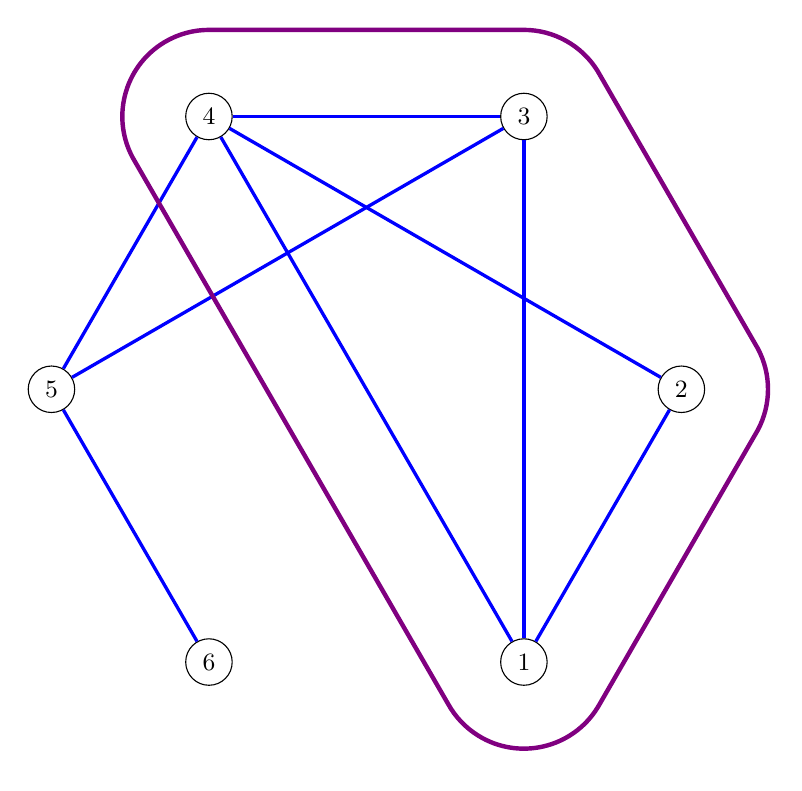
\begin{tikzpicture}
\def \n {6}
\def \radius {4cm}
\def \margin {8} % margin in angles, depends on the radius
\foreach \s in {1,...,6}
{
{\node[draw, circle] (\s) at ({360/\n * (\s - 2)}:\radius)  {\small $\s$};}
} 
\draw [color=blue,very thick] (1) -- (2) ; 
\draw [color=blue,very thick] (4) -- (2) ; 
\draw [color=blue,very thick] (1) -- (3) ; 
\draw [color=blue,very thick] (1) -- (4) ; 
\draw [color=blue,very thick] (4) -- (5) ; 
\draw [color=blue,very thick] (3) -- (5) ; 
\draw [color=blue,very thick] (6) -- (5) ; 
\draw [color=blue,very thick] (3) -- (4) ; 

 % \draw[green,ultra thick] \convexpath{1,5,4,3,2}{1.4cm};
% \draw[yellow,very thick] \convexpath{1,6, 4,3,2}{1.7cm};
\draw[violet,ultra thick] \convexpath{1,4,3,2}{1.1cm};
\end{tikzpicture}} &
\fbox{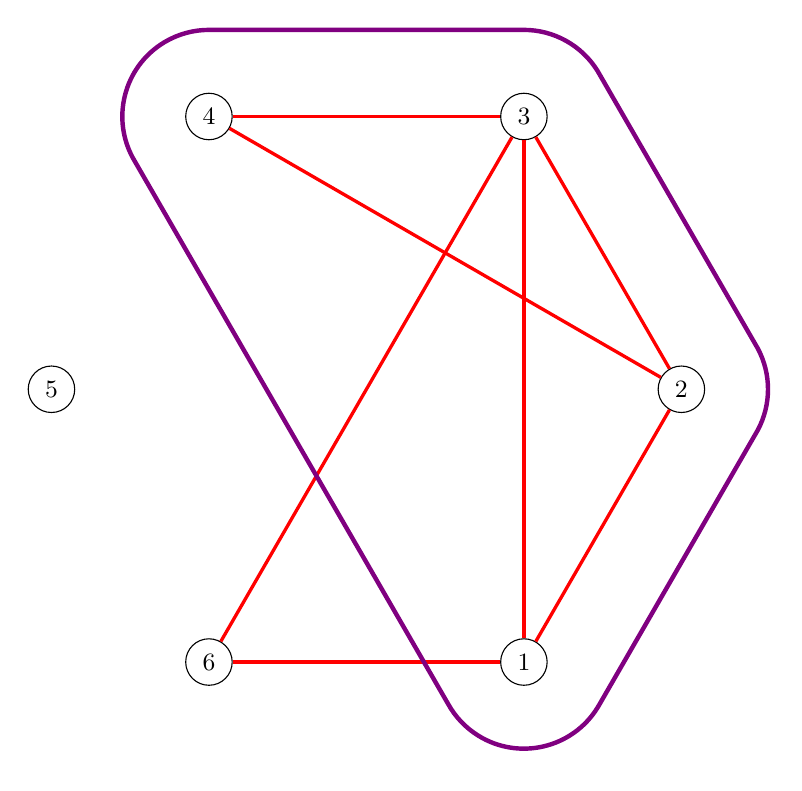
\begin{tikzpicture}
\def \n {6}
\def \radius {4cm}
\def \margin {8} % margin in angles, depends on the radius
\foreach \s in {1,...,6}
{
\node[draw, circle] (\s) at ({360/\n * (\s - 2)}:\radius) {\small $\s$};
} 
\draw [color=red,very thick] (1) -- (2)  ; %node [near end, below=5pt] {\Large\textcolor{red}{$x^{(2)}_{12}$}}; 
\draw [color=red,very thick] (3) -- (2)  ; % node [near end, above=10pt] {\Large\textcolor{red}{$x^{(2)}_{23}$}}; 
\draw [color=red,very thick] (1) -- (3)  ; % node [midway, below=10pt] {\Large\textcolor{red}{$x^{(2)}_{13}$}}; 
\draw [color=red,very thick] (4) -- (2)  ; % node [near start, below=2pt] {\Large\textcolor{red}{$x^{(2)}_{24}$}}; 
\draw [color=red,very thick] (3) -- (4)  ; % node [midway, above=1pt] {\Large\textcolor{red}{$x^{(2)}_{34}$}}; 

\draw [color=red,very thick] (1) -- (6)  ; % node [midway, below=1pt] {\Large\textcolor{red}{$x^{(2)}_{16}$}}; 
\draw [color=red,very thick] (3) -- (6)  ; % node [midway, below=2pt] {\Large\textcolor{red}{$x^{(2)}_{36}$}}; 
%  \draw[green,ultra thick] \convexpath{1,5,4,3,2}{1.4cm};
% \draw[yellow,very thick] \convexpath{1,6, 4,3,2}{1.7cm};
\draw[violet,ultra thick] \convexpath{1,4,3,2}{1.1cm};
\end{tikzpicture}} & 

\raisebox{0.4\totalheight}{\parbox[t]{0.3\linewidth}{\begin{tabular}[c]{l|ll|l }
       \hline $S$ & \textcolor{blue}{$\delta^{(1)}$} & \textcolor{red}{$\delta^{(2)}$} & $\delta^{\min}$  \\\hline 
 {123456} & $1.33$ & $1.17$ & $1.17$\\        
\textcolor{black}{12345} & $1.4$ & $1.0$   & $1.0$\\ 
\textcolor{black}{$12346$} & $1.0$ & $1.4$  & $1.0$\\  
     \textcolor{violet}{$1234$} & $1.25$ & $1.25$    & $1.25$ \\
{$\vdots$} & $\vdots$ & $\vdots$  & $\vdots$\\ \hline
\multicolumn{3}{r}{$\delta_{DCS} = $} & $1.25$
\end{tabular}
% \begin{align*} \delta_{DCS} & = \max \delta^{\min}(S) \end{align*}
}} 
\end{tabular}

\end{center}
}